\documentclass{book}
\usepackage{polyglossia}  % Hyphenation
\setmainlanguage{english}
\usepackage{minted}       % Source code typesettings
\setminted{breaklines=true}
\usepackage{placeins}     % Float barriers
\usepackage{tikz}         % Diagrams
\usetikzlibrary{trees,arrows}
\usepackage{fancyvrb}     % Manually colored verbatim
\usepackage{float}        % Non-floating figures
\usepackage{./main}
\title{Electronic Document Preparation: An Author's Cookbook}
\author{Vít Novotný}
\date{\today}
\begin{document}
  \frontmatter
    \maketitle
    \tableofcontents
  \mainmatter
    \chapter{Foreword}
      With the advent of the digital age, typesetting has become available to
      virtually anyone equipped with a personal computer. Beautiful documents
      can now be crafted using free and consumer-grade software, which often
      obviates the need for the involvement of a professional designer and
      typesetter. The level playing field of the Internet coupled with the
      rising popularity of digital-only documents then allows the aspiring
      author to bypass the publisher as well, if they so wish, without
      jeopardizing their chance of recognition.
      
      This text is intended as a handbook for any author who aspires to write,
      design, typeset and distribute high-quality documents of their own making.
      Each chapters describes one discrete step of document creation along with
      the relevant tools and literature. Since document preparation is a broad,
      multidisciplinary subject, the main goal of this text is to provide the
      reader with a general overview of the landscape and to provide references
      to more detailed literature for those interested in further study.

    \chapter{Writing}
      % Text encodings
      % Text editors
      % Regular expressions
      % Versioning systems

    \chapter{Markup}
      A manuscript can consist of a seamless river of words and still make
      perfect sense to the author. To truly capture its meaning in a clear and
      unambiguous manner, however, the manuscript will often need to be
      supplemented with a set of annotations. At a more basic level, this refers
      to the compliance with the orthographic rules, such as the correct
      spelling, hyphenation, capitalization, word breaks and punctuation, that
      are specific to the language of the document. It is not at all
      unreasonable to expect that this basic compliance should be already met by
      the manuscript.  At a higher level, this consists of discovering and
      marking up the inner order and the logic of the text, so that the
      resulting document can later be typeset in a way that visually reflects
      the structure of the text.
      
      To this end, there exists a wealth of \emph{markup languages} that enable
      the enrichment of text with additional information and labels. Aside from
      \emph{logical markup}, which enables the capture of the logical structure
      of the document, markup languages may also provide \emph{presentation
      markup}, which directly impacts the visual properties of the document, but
      carries no semantic information. The usage of presentation markup instead
      of logical markup makes it impossible to separate the markup from the
      design of the document and to capture the logic of the text. As a result,
      the unity in the design of each logical part of the document would have to
      be ensured manually and future changes of design would become tedious. It
      is for these reasons that the usage of presentation markup is discouraged
      in favour of logical markup.

      \section{Meta Markup Languages}
      \subsection{The General Markup Language}
        The situation engulfing digital typesetting was growing increasingly
        frustrating for publishers in the 1960s. The markup languages used by
        different typesetting systems varied wildly and once a publisher had a
        large collection of documents typeset via a given company, switching to
        another one could be very costly venture. The companies would often take
        advantage of this situation, causing their prices to skyrocket. As a
        result of that, a demand for a universal markup language emerged.

        This demand was met by a project developed\footnote{
          More information about the project can be found within the personal
          recollections of its co-author, Charles F. Goldfarb, in
          \cite{goldfarb96} and \cite{goldfarb97:whySGML}.
        } at the \acronym{IBM}'s Cambridge Scientific Center in the early 1970s.
        The project aimed at imbuing a text editor with the ability to query,
        edit and display documents from a repository to allow the usage of
        computers in legal practice. Very early on in the development process,
        it became clear that the crux was going to be the markup languages in
        which the documents were written. These languages were not unified and
        many of them comprised largely presentation markup, which made
        information retrieval impossible without the use of heuristics. To
        resolve the issue, a unifying markup language called the General Markup
        Language (\acronym{GML}) was drafted as a solution to the described
        problem. The language was later released to the public in
        \cite{goldfarb81} and finally standardized\footnote{
          The authoritative resource on the \acronym{SGML} language is
          \cite{goldfarb91}, which includes the full text of the standard along
          with the author's extensive annotations.
        } as the Standard General Markup Language (\acronym{SGML}) within
        \cite{iso8879}.

        \acronym{SGML} documents consist of text mixed with \emph{tags}, which
        delimit meaningful sections of the document called \emph{elements}.
        Elements can carry additional information in \emph{attributes}.
        Additionally, \acronym{SGML} document can contain miscellaneous
        instructions for the program that is processing it, as well as
        human-readable comments. Repeated strings of text can be declared as
        \emph{entities} that can consequently be used throughout the document in
        place of the original strings.
        
        Although the described structure is shared by all \acronym{SGML}
        documents, the actual syntax, as well as the restrictions with regards
        to the contents and the attributes of individual elements, are declared
        within a Document Type Declaration (\acronym{DTD}), which can be
        different for each document. It is worth noting that a \acronym{DTD}
        only declares the syntax of an \acronym{SGML} document and the semantics
        of the individual elements and their attributes are left to the
        interpretation of the program processing the document. The syntax and
        the constraints imposed by a \acronym{DTD} define an \emph{application}
        of \acronym{SGML}. An \acronym{SGML} document is considered to be a
        valid instance of an \acronym{SGML} application, when it conforms to the
        respective \acronym{DTD}.

      \subsection{The Extensible Markup Language}
        Although \acronym{SGML} was designed to be the general format for data
        exchange, the complexity of the specification and the lack of support
        for Unicode proved to be a major hindrance preventing its wider
        adoption and tool development. As a response, the World Wide Web
        Consortium (W3C) published a specification of the Extensible Markup
        Language (\acronym{XML}) within \cite{bray98} in 1998. Along with the
        introduction of \acronym{XML}, the \acronym{SGML} specification received
        a technical corrigendum of \cite{goldfarb97:webSGML}, which turned
        \acronym{XML} into a proper subset of \acronym{SGML} restrained by an
        \acronym{SGML} \acronym{DTD}.
        
        \begin{figure}
          \inputminted{xml}{examples/02/recipe.xml}
          \caption{An example \acronym{XML} document\filename{recipe.xml}}
          \label{fig:recipe}\bigskip
          \inputminted{dtd}{examples/02/dtdtypes}
          \caption{\acronym{SGML} and \acronym{XML} \acronym{DTD}s can be either
            linked to the document through public and system identifiers, directly
            embedded in the document, both linked and embedded or left out
            altogether.}
          \label{fig:recipe-dtd}
        \end{figure}
        
        This \acronym{DTD} completely fixes the syntax of \acronym{XML}
        documents, which makes it possible to differentiate two levels of
        correctness. Specifically, an \acronym{XML} document is considered to be
        \emph{well-formed}, when it conforms to the \acronym{SGML} \acronym{DTD}
        that restrains \acronym{XML} as well as to the additional constraints
        given in the specification. An \acronym{XML} document is considered to
        be \emph{valid} against an \acronym{XML} \acronym{DTD}, when it
        is well-formed and conforms to the said \acronym{XML} \acronym{DTD}.
        Along with \acronym{DTD}s, there exists\footnote{
          A list of tools for the manipulation of files in \acronym{XML} schema
          languages is maintained on the web site of \acronym{W3C} at
          \url{http://www.w3.org/XML/Schema}.
        } a wealth of \emph{schema} languages for \acronym{XML}, such as
        \acronym{W3C XML} Schema, Regular Language for \acronym{XML} Next
        Generation (\acronym{Relax NG}) or Schematron that can be used to check
        the validity of an \acronym{XML} document instead of a \acronym{DTD}.
        The constrains imposed by either a \acronym{DTD} or a schema define an
        \emph{application}, \emph{language} or \emph{format} of \acronym{XML}.

        Along with schema languages, other supplementary languages also exist,
        such as XPointer, XPath and XQuery for addressing sets of elements
        (fragments) within a \acronym{XML} document or Cascading Style Sheet
        language (\acronym{CSS}) for specifying the visual properties of an
        \acronym{XML} document. While some of these languages may not be
        \acronym{XML} languages, they are nevertheless used within documents of
        various \acronym{XML} formats and form an important part of the
        \acronym{XML} ecosystem.

        A notable new feature of \acronym{XML} are \emph{namespaces}, which
        were added to the specification with the release of \cite{bray99} in
        1999. Namespaces enable the inclusion of elements and attributes of
        different \acronym{XML} applications within a single \acronym{XML}
        document by providing a method to qualify element and attribute names
        with Internationalized Resource Identifiers (\acronym{IRI}s)---specified
        within \cite{rfc3987}---that uniquely represent the respective
        \acronym{XML} applications. Namespaced elements are a spiritual
        successor of a more expressive \acronym{SGML} feature of
        \texttt{CONCUR}, which makes it possible to mark up several structural
        views of a single document. Unlike with \texttt{CONCUR}, which ties each
        view to an \acronym{SGML} \acronym{DTD}, there exists no general
        mechanism for the translation of \acronym{IRI}s to \acronym{XML}
        schemata. This makes it impossible to validate namespaced \acronym{XML}
        documents, unless all the \acronym{IRI}s and the respective schemata are
        known to the parser.

        \begin{figure}[hb!]
          {\tikzstyle{level 1}=[sibling distance=\baselineskip, level distance=1.5cm]
\begin{tikzpicture}[grow=right]
  \node {\textcolor{red}{Speech}}
    child {
      node [label=right:{AASE: See, you dare not! Every word of it's a
        lie!} ] {}}
    child {
      node[label=right:{PEER: Swear? Why should I?}] {} }
    child {
      node[label=right:{AASE: Well then, swear to me it's true!}] {}}
    child {
      node[label=right:{PEER: No, I'm not!}] {} }
    child {
      node[label=right:{AASE: Peer, you're lying!}] {} };
  \node [below=5\baselineskip] {\textcolor{blue}{Verse}}
    child {
      node[label=right:{Every word of it's a lie!} ] {}}
    child {
      node[label=right:{Swear? Why should I? See, you dare not!}] {} }
    child {
      node[label=right:{Well then, swear to me it's true!}] {}}
    child {
      node[label=right:{Peer, you're lying! No, I'm not!}] {} };
\end{tikzpicture}}%
\begin{Verbatim}[commandchars=\\\{\},codes={\catcode`$=3\catcode`^=7\catcode`_=8}]
<(\textcolor{blue}{V})line>
  <(\textcolor{red}{S})speech who="Aase">Peer, you're lying!</(\textcolor{red}{S})speech>
  <(\textcolor{red}{S})speech who="Peer">No, I'm not!</(\textcolor{red}{S})speech>
</(\textcolor{blue}{V})line><(\textcolor{blue}{V})line>
  <(\textcolor{red}{S})speech who="Aase">Well then,
    swear to me it's true!</(\textcolor{red}{S})speech>
</(\textcolor{blue}{V})line><(\textcolor{blue}{V})line>
  <(\textcolor{red}{S})speech who="Peer">Swear, why should I?</(\textcolor{red}{S})speech>
  <(\textcolor{red}{S})speech who="Aase">See, you dare not!
</(\textcolor{blue}{V})line><(\textcolor{blue}{V})line>
  Every word of it's a lie!</(\textcolor{red}{S})speech>
</(\textcolor{blue}{V})line>
\end{Verbatim}

          \caption{The markup of the dramatic and metrical views of the
            beginning of Henrik Ibsen's \work{Peer Gynt} using the
            \texttt{CONCUR} feature of \acronym{SGML}}
        \end{figure}

        %%% Živoucí CONCAT <http://webylon.info/K.24>
        %%% Popis SGML deklarace pro ISO/IEC15445
        %%%   <http://www.angelovic.cz/internet/sgml-deklarace.html#concur>

        \begin{figure}[H]
          \inputminted{xml}{examples/02/recipe.xsd}
          \caption{A reformulation of the recipe \acronym{DTD} from Figure
            \ref{fig:recipe-dtd} in the \acronym{XML} Schema language.%
            \filename{recipe.xsd}}
          \label{fig:recipe-xsd}
          \inputminted{text}{examples/02/recipe.rnc}
          \caption{A reformulation of the recipe \acronym{DTD} from Figure
            \ref{fig:recipe-dtd} in the compact syntax of the \acronym{Relax NG}
            language.\filename{recipe.rnc}}
          \label{fig:recipe-rnc}
          \inputminted{sh}{examples/02/recipe.sh}
          \caption{\acronym{XML} documents can be easily validated against
            \acronym{XML} schemata using command-line tools, such as
            \texttt{xmllint}.}
        \end{figure}

        Due to the reduced complexity of \acronym{XML} compared to
        \acronym{SGML}, the language was adopted by specialists and the general
        public alike and has superseded \acronym{SGML} in many applications.
        Some of the applications of \acronym{XML} for document
        preparation include DocBook\footnote{
          The authoritative resource on the DocBook \acronym{XML} format is
          \cite{walsh10}. The book itself is written in DocBook and its source
          code is publicly available at the Web page at
          \url{http://docbook.org}.
        }---a technical documentation format used for authoring books by
        publishers such as O'Reilly Media and for documenting software at
        companies such as Red Hat, \acronym{SUSE} or Sun Microsystems---,
        Text Encoding Initiative (\acronym{TEI})---a general text encoding
        format for the use in the academic field of digital humanities---,
        Mathematical Markup Language (\acronym{MathML})---a format for
        describing mathematical formulae---, or Scalable Vector Graphics
        (\acronym{SVG})---a two-dimensional vector image format. Other
        \acronym{XML} applications, such as \acronym{XHTML} and
        \acronym{RDF/XML}, will be discussed in Section \ref{sec:www-markup}.
      
      \section{Markup on the World Wide Web}\label{sec:www-markup}
      \subsection{The Hypertext Markup Language}
        In 1989, Timothy John Berners-Lee proposed in \cite{bernerslee89} a
        decentralized system for sharing linked documents within \acronym{CERN}.
        The system laid foundation for today's World Wide Web (Web) and earned
        its author knighthood. The markup language used to write documents for
        the system was an application of \acronym{SGML} called the HyperText
        Markup Language (\acronym{HTML}). In 1993, the Web started to gain
        popularity amongst the general public due to the release of the first
        graphical Web browser Mosaic, which paved way for the Web browsers of
        today. In 1994, Timothy John Berners-Lee formed the World Wide Web
        Consortium (\acronym{W3C}), which has since been developing the
        standards for the Web.
        
        The first standard version of \acronym{HTML} was version 2.0 published
        as \cite{rfc1866} in 1995. As the Web was becoming ubiquitous, it began
        accumulating an increasing number of documents that weren't valid
        instances of \acronym{HTML}, since most Web browsers, when faced with a
        malformed document, would act in accordance with the Postel's law and
        try to render the document despite its deficiencies. In an attempt to
        unify the way malformed \acronym{HTML} documents were rendered across
        the Web browsers, \acronym{W3C} acknowledged and documented this
        behaviour as a part of \cite[Section~8.2, Parsing HTML
        documents]{hickson14} in 2008. An example is presented in Figure
        \ref{fig:overlapping-elements}.

        \begin{figure}[b]
          \begin{minted}[linenos]{html}
            <b>This text is bold, <i>bold and italic</b>, italic.</i>
            <b>This text is bold, </b><i><b>bold and italic</b>, italic.</i>
          \end{minted}
          \caption{The fragment on line 1 contains overlapping elements and as
            such, it can't be a part of a valid \acronym{HTML} document.
            However, it is recommended by \acronym{W3C} that browsers should
            parse the fragment identically to the fragment on line 2.}
          \label{fig:overlapping-elements}
        \end{figure}

        Initially, \acronym{HTML} comprised a mixture of logical and
        presentation markup with fixed visual interpretation. In 1996, a
        specification of a Cascading Style Sheet (\acronym{CSS}) language was
        published by \acronym{W3C} within \cite{lie96}. The language enabled
        the specification of the visual properties of any element, which allowed
        for the separation of document markup and design, effectively
        eliminating the need for the presentation markup.

        \begin{figure}
          \inputminted{html}{examples/02/presentation-markup.html}
          \caption{An excerpt from the Web site of the \acronym{CSS} Zen Zarden
            located at \protect\url{http://csszengarden.com}. The document above
            was created using the \acronym{HTML} presentation markup. The
            document below achieves the same appearance by the combination of
            logical markup and \acronym{CSS} definitions.}\medskip
          \inputminted{html}{examples/02/logical-markup.html}
        \end{figure}

        During the same period, an initial version of a scripting language
        called JavaScript was drafted and incorporated into Netscape Navigator
        2.0, one of the contemporary leading web browsers and a descendant of
        the original Mosaic browser. As a part of a joint effort to bring Java
        into web browsers by Sun Microsystems and Netscape Communications,
        JavaScript was, according to \cite{js-announcement}, supposed to
        complement Java applets -- a role it has since outgrown. Standardized
        within \cite{ecma1} in 1997, JavaScript blurs the line between static
        documents and interactive applications and remains the predominant
        client-side programming language for the Web.  However, since the
        support of JavaScript by a Web browser is fully optional, it is
        considered a good practice to use it chiefly for the enrichment of
        already self-sufficient \acronym{HTML} documents. In case of an
        interactive application, this recommendation can be relaxed.

      \subsection{The Extensible Hypertext Markup Language}
        Ever since the release of \acronym{XML} in 1998, \acronym{W3C}
        entertained the idea of turning \acronym{HTML} into an application of
        \acronym{XML}, rather than \acronym{SGML}, as exemplified by the working
        draft of \cite{raggett98} released the very same year. Unlike
        \acronym{HTML} parsers, which are complex in their acceptance of
        malformed content, \acronym{XML} parsers are, as per \cite[Section~1.2,
        Terminology]{bray98}, required to draconianly refuse \acronym{XML}
        documents that aren't well-formed, leading to architectural simplicity
        and decreased computational requirements. As a result, reformulating
        \acronym{HTML} in \acronym{XML} was suggested as a way to bring the Web
        to mobile, embedded and other devices limited in their resources, as
        well as to reduce the amount of malformed documents on the Web in
        general. Other perceived advantages included the ability to use
        \acronym{XML} tools for web documents and to include instances of other
        \acronym{XML} applications, such as \acronym{MathML} and \acronym{SVG},
        directly into web documents using \acronym{XML} namespaces.

        The idea was brought to fruition within \cite{pemberton00} in 2000 as an
        \acronym{XML} application called the Extensible HyperText Markup
        Language (\acronym{XHTML}), which was met with lukewarm reception, since
        many of its supposed benefits proved to be either questionable or too
        marginal to warrant migration from \acronym{HTML}.  The speed advantages
        of the simpler parser were largely offset by its lack of support for
        incremental rendering, caused by the impossibility to validate partially
        downloaded pages, the closing of the gap in the computing power between
        mobile and desktop devices made it possible to use full-fledged
        \acronym{HTML} parsers across the spectrum, and the lack of ways to
        provide alternative content for browsers that would not support directly
        included the \acronym{XML} documents considerably reduced the usefulness
        of \acronym{XML} namespaces. As a result, \acronym{XHTML} has yet to
        succeed in replacing \acronym{HTML} and remains an alternative markup
        language for the Web.
        
        %%% Content-Negotiation Techniques to serve XHTML as text/html and
        %%% application/xhtml+xml
        %%%   <http://www.w3.org/2003/01/xhtml-mimetype/content-negotiation>

      \subsection{The Semantic Web and Linked Data}
        The underlying fundament of the Web is the the idea of a globally
        available and incrementally scalable base of human knowledge.
        \acronym{HTML} and \acronym{XHTML} succeeded in fulfilling this vision
        for human-readable documents, but didn't provide a unifying
        machine-readable format for the representation of structured information
        that would enable the creation of a web of linked data running in
        parallel to the web of documents. In 1999, \acronym{W3C} released
        \cite{lassira99} containing the specification of the Resource
        Description Framework (\acronym{RDF}), a method for the description of
        resources on the Web.

        Drawing from the research in the field of knowledge representation, an
        \acronym{RDF} document represents data as a set of \emph{triples}. Each
        of the triplets comprises \emph{a predicate}, \emph{a subject} and
        \emph{an object}, where both the predicate and the subject are specified
        as \emph{resources} using \acronym{IRI}s. If the object of a
        triplet $(p,s,o)$ is also a resource, the triplet can be interpreted as
        a subject $s$ being in a relation $p$ with the object $o$. If the object
        is a \emph{literal value} rather than a resource, the respective triplet
        can be interpreted as a subject $s$ having a property $p$ with the value
        $o$.

        Resources in \acronym{RDF} are specified via \acronym{IRI}s to prevent
        naming collisions in \acronym{RDF} documents created independently by
        distinct authors. These \acronym{IRI}s are not required to resolve to an
        actual web page and, disregarding the small set of standard resources
        specified within the \acronym{RDF} specification, they carry no
        inherent meaning.  In order to describe a set of resources, the
        relationships between them, and their intended meaning in an
        \acronym{RDF} document, an extension of the set of standard resources%
        ---called \acronym{RDF} Schema and specified within
        \cite{brickley04}---can be used.  The resulting documents are called
        \emph{ontologies} and can be used for automated reasoning about
        \acronym{RDF} documents containing resources described by the
        ontology.\footnote{
          A list of ontologies that are fully documented, honor the current best
          practices and are supported by various tools can be found on the
          \acronym{W3C} wiki at \url{http://www.w3.org/wiki/Good_Ontologies}.
        } Some of the well-known ontologies include Dublin
        Core (\acronym{DC})---an ontology for the generic description of both
        web multimedia and physical objects---, Friend or a Foe
        (\acronym{FOAF})---an ontology for the description of people and their
        social relationships---, or the Music Ontology---an ontology for the
        description of entities related to the music industry, such as albums,
        artists, tracks and events. More expressive standards for the creation
        of ontologies, such as the Web Ontology Language (\acronym{OWL})
        specified within \cite{mcguinness04}, also exist.

        The syntax of \acronym{RDF} is not fixed, meaning that aside from the
        \acronym{XML} serialization specified within \cite{lassira99}, other
        languages, such as the JavaScript Object Notation for Linked Data
        (\acronym{JSON-LD}) specified within \cite{sporny14}, the Turtle
        language specified within \cite{beckett14-turtle}, or the line-based
        N-Triples language specified within \cite{beckett14-nt}, can be used to
        represent an \acronym{RDF} document. A noteworthy serialization of
        \acronym{RDF} is the \acronym{RDF} in attributes (\acronym{RDFa})
        specified within \cite{adida08}. While various serializations of
        \acronym{RDF} can be included in or linked to an \acronym{HTML} or
        \acronym{XHTML} document, this will often result in an undesirable
        duplication of data already present in the document. To prevent this,
        \acronym{RDFa} uses the content already present within the underlying
        \acronym{HTML} or \acronym{XHTML} document using element attributes. The
        usage of \acronym{RDF} in conjunction with \acronym{HTML} and
        \acronym{XHTML} is intended to gradually obsolete the practice of using
        the \texttt{meta} and \texttt{link} elements to provide additional
        application-specific metadata about the document.

        \begin{figure}
          \inputminted{xml}{examples/02/john.rd}
          \inputminted{text}{examples/02/john.nt}
          \inputminted{text}{examples/02/john.ttl}
          \caption{Above is an example \acronym{RDF} document using \acronym{DC}
            and \acronym{FOAF} ontologies in the \acronym{RDF}/\acronym{XML}%
            \filename{john.rd}, N-Triples\filename{john.nt} and Turtle%
            \filename{john.ttl} serializations. Below is a graph representation
            of the document.}\label{fig:rdf-doc}\bigskip
          {\tikzstyle{level 1}=[sibling distance=6\baselineskip, level distance=0.5cm]
\tikzstyle{level 2}=[sibling distance=6\baselineskip, level distance=0.5cm]
\centerline{\begin{tikzpicture}[grow=right,->]
  \node[label=left:{\url{http://example.org/document.html}}] {}
    child { node {\texttt{"The Web page of John Smith"@en}}
      edge from parent
      node[left] {\textcolor{blue}{dc:title}}}
    child { node {\url{http://example.org/john-smith}}
      child { node[label=right:{foaf:Person}] {}
        edge from parent
        node[right,align=left] {\textcolor{blue}{rdf:type}}}
      child { node {\texttt{"John Smith"}}
        edge from parent
        node[left] {\textcolor{blue}{foaf:name}}}
      edge from parent
      node[left] {\textcolor{blue}{foaf:creator}};
    };
\end{tikzpicture}}}

        \end{figure}

        \begin{figure}[t!]
          \inputminted{html}{examples/02/john.html.linked-rdf}
          \caption{Above is an \acronym{HTML} document linked to the
            \acronym{RDF} document from Figure \ref{fig:rdf-doc}. Below is the
            same \acronym{HTML} document with the \acronym{RDF} data directly
            embedded using the \acronym{RDFa} serialization.}\bigskip
          \inputminted{html}{examples/02/john.html.rdfa}
        \end{figure}

        %%% Tim Berners-Lee: The next web
        %%%   <http://www.ted.com/talks/tim_berners_lee_on_the_next_web>
        %%%
        %%% The SPARQL Query Language for RDF (SPARQL) and the (at the time of
        %%% writing only drafted) Linked Data Fragments RDF query interfaces
        %%%   <http://www.w3.org/TR/rdf-sparql-query/>
        %%%   <http://linkeddatafragments.org/specification/>
        %%%
        %%% The Rule Interchange Format (RIF)
        %%%   <http://www.w3.org/TR/rif-overview/>
        
      \section{Markup in Document Processing Systems}
        Some of the existing markup is directly tied with specific document
        preparation systems. These can be dichotomized into batch-oriented
        systems, which process marked up input text documents into printable
        output documents in a page description language on demand, and
        interactive systems, which allow the user to directly edit an
        approximation of the output document via a visual editor. Also referred
        to as \emph{What You See Is What You Get} (\acronym{WYSIWYG}),
        interactive systems exchange mild learning curve for more primitive
        typesetting algorithms, which don't stand in the way of interactivity,
        and for reduced flexibility stemming from the usage of a Graphical User
        Interface (\acronym{GUI}), which, although often intuitive for simple
        tasks, seldom matches the power of markup languages used by
        batch-oriented systems.

      \subsection{Batch-oriented Document Preparation Systems}
        One of the archetypal batch-oriented systems are \texttt{troff} and
        \texttt{nroff} from 1970s, which were available for \acronym{UNIX}
        operating systems and which were used to produce output for either
        general printers or line printers and terminals, respectively. A free
        alternative from \acronym{GNU} called \texttt{groff} combines the
        capabilities of both \texttt{troff} and \texttt{nroff}, and is used
        extensively to date for the markup of documentation in \acronym{UNIX}
        and \acronym{UNIX}-like operating systems, although more advanced
        alternatives exist for general typesetting. The associated markup
        language combines presentation markup with programming constructs and
        allows the definition of logical markup in the form of user macros.
        Standard macro packages, such as \texttt{man} for the formatting of
        documentation, \texttt{me} for the creation of research papers, or
        the more recent \texttt{mom} for general typesetting tasks are
        typically distributed along with the system. Special markup invokes
        preprocessors, which can be used for the typesetting of tables,
        equations and vector graphics.

        \begin{figure}
          \fbox{\includegraphics[clip,trim=1.7cm 12cm 1.7cm 1.3cm,%
            width=0.975\textwidth]{examples/02/poe-groff.pdf}}
          \inputminted{groff}{examples/02/poe.groff}
          \caption{An excerpt from the beginning of Edgar Allen Poe's
            \work{Cask of Amontillado} formatted using the \texttt{mom}
            macro package of \texttt{groff}.}
          \label{fig:poe}
        \end{figure}

          %%% The Groff and Friends HOWTO
          %%%   <http://troff.org/TheGroffFriendsHowto.pdf>
          %%%
          %%% Writing Macros
          %%%   <https://www.gnu.org/software/groff/manual/html_node/Writing-Macros.html>

        Another notable batch-oriented system is \TeX\footnote{
          The circumstances that led to the creation of \TeX\ and the
          surrounding tools are thoroughly documented in \cite{knuth98}.
        }, which was developed and consequently released to the public domain by
        in 1970s a professor of computer science Donald Knuth, after he had
        received galley proofs for the second volume of his monograph, the Art
        of Computer Programming, and found the appearance of mathematical
        formulae unsatisfactory. As a result, the typesetting of mathematics is
        a central theme in \TeX, rather than an afterthought, which
        differentiates it from most other document preparation systems and
        largely attributed to the massive popularity it attained in academia.
        Much like in the case of \texttt{troff} and its derivatives, the
        language of \TeX\ is ripe with typographic and programming primitives
        and doesn't by itself contain logical markup. The language, however,
        allows for the creation of user macros. An example of a macro package,
        which makes it possible to create various classes of documents with pure
        logical markup, is \LaTeX, the industry standard for academic and
        technical typesetting.
        
        \begin{figure}
          \inputminted{tex}{examples/02/poe.tex}
          \caption{The \texttt{groff} document from Figure \ref{fig:poe}
            reformulated using \TeX}
        \end{figure}

      \subsection{Interactive Document Preparation Systems}
        Interactive systems come in two distinctive flavours. \emph{Word
        processors} are the digital progeny of the typewriter machine, with
        which they share the main function of fast text capture. The typewriter
        output documents served largely as a manuscript for designers and
        typographers, who then produced the actual published work. With the
        advent of personal computing and the Web, self-publishing became more
        approachable to the general public and modern word processors can be
        used not only to write, but also to design and set typeset documents,
        although the offered functionally is typically constrained by user
        experience demands. This concern is not shared by \emph{desktop
        publishing software}, which provides refined control over the resulting page
        layout and the typesetting primitives at the expense of steeper learning
        curve, but with the ability to produce document comparable to those set
        using traditional typography.

        Most interactive systems will provide a means to mark up sections of
        text. Presentation markup performs direct changes of typographic
        properties, such as the face, family, variant, color or the size
        of the font that is used to typeset the text. Logical markup enables
        the classification of sections of text with the ability to set up the
        design of each class later on. This decouples writing and markup from
        design and makes it easy to change the design of the entire document and
        difficult to produce inconsistent design.

        \begin{figure}
          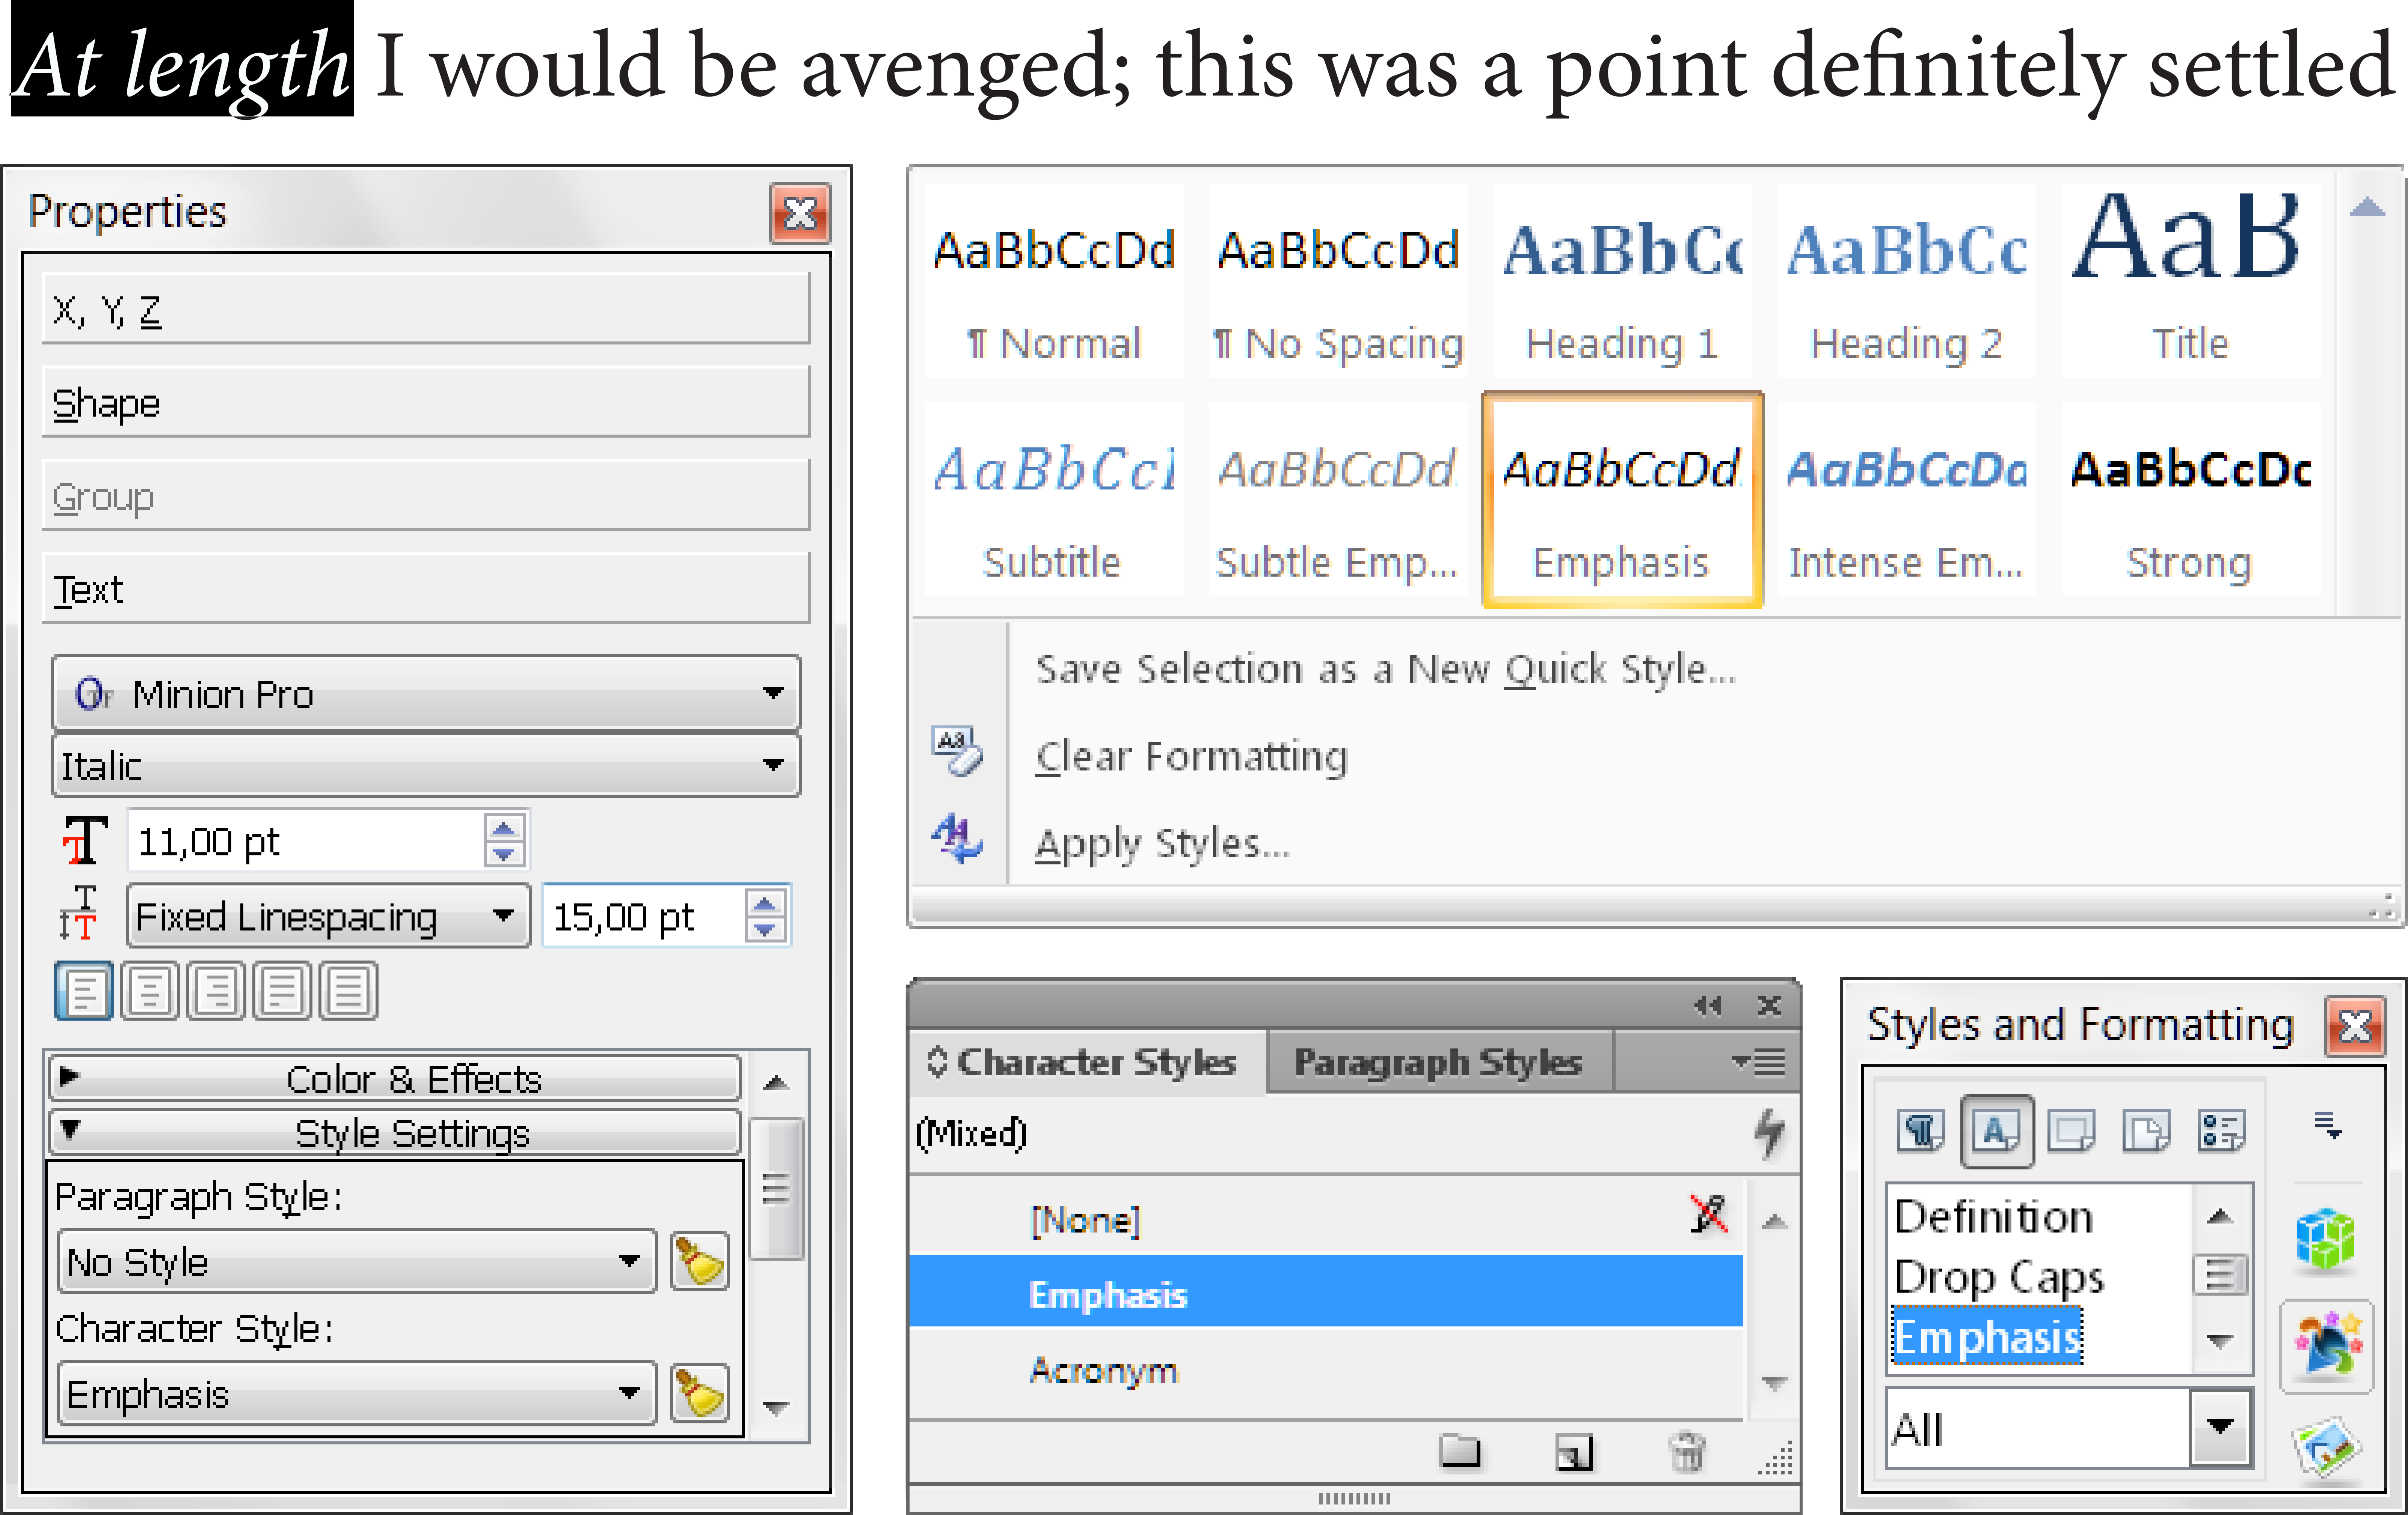
\includegraphics[width=\textwidth]{examples/02/interactive-editors.png}
          \caption{Logical markup in the interactive document preparation
            systems of Scribus (left), Microsoft Word (above), Adobe InDesign
            (below left) and Apache OpenOffice (below right)}
        \end{figure}
          % An example of Word, OpenOffice, Indesign and Scribus markup

        % WYSIWYG
          % Word, OpenOffice, Adobe InDesign, Scribus
          %%% Style basics in Word <https://support.office.com/en-nz/article/Style-basics-in-Word-d382f84d-5c38-4444-98a5-9cbb6ede1ba4>
          %%% InDesign Help / Paragraph and character style <https://helpx.adobe.com/indesign/using/paragraph-character-styles.html>
          %%% Format text with Paragraph Styles <https://helpx.adobe.com/indesign/how-to/indesign-formatting-text-paragraph-styles.html>

      \section{Lightweight Markup Languages}
        Parallel to the heavy-duty applications of \acronym{SGML} and
        \acronym{XML}, there runs a vein of markup languages that give priority
        to unobtrusiveness and legibility over expressiveness and genericity.
        Rooted in the reality of computer text terminals with limited formatting
        capabilities, lightweight markup languages leverage symbols and
        indentation to produce comparatively weak and domain-specific, but also
        humane, highly intuitive and often profoundly beautiful markup that is
        easy to both read and write. Examples of lightweight markup languages
        include Markdown, Creole, AsciiDoc, MakeDoc, Setext or Wikicode.
        Lightweight markup languages are typically supplemented by tools, which
        enable the conversion to more general languages, such as \acronym{HTML}.
        Also typical is the existence of numerous flavours of every lightweight
        markup language, which represent different use cases.

    \chapter{Design}
      % XML -- CSS, XSL, XSLT
    \chapter{Typesetting}
    \chapter{Proofreading}
    \chapter{Printing}
    \chapter{Distribution}
\end{document}
